\chapter{Monte Carlo Methods}


We begin this chapter with a recapitulation of part of the lecture held in the past Semester, \emph{Introduction to Computational Physics} (ICP). Basic knowledge of statistical physics as well as a certain acquaintance with the content of ICP is assumed. For more information about the mentioned lecture and detailed derivation of some of the formulae contained in this chapter, see  \citet{comp_phys}.

\vspace{.4cm}
\noindent
After a brief definition of some basic concept in statistical physics (\textbf{phase space}, \textbf{micro-} and \textbf{canonical ensembles}), the \textbf{Ising model} is introduced with some important concepts and observables (\textbf{order parameter}, \textbf{response functions}, \textbf{fluctuation-dissipation theorem}, \textbf{correlation length} and \textbf{critical exponents}). In the second and third part, \textbf{Monte Carlo} and \textbf{finite size} methods are treated respectively. Those who attended ICP will find that some parts are already familiar to them. The last three sections of the chapter (\textbf{cluster algorithms}, \textbf{histogram methods} and \textbf{renormalization}) contain some optimization and generalization of MC and were not treated in ICP. 

\section{Classical Statistical Physics}

\subsection{Phase Space}
Let us consider a classical physical system with N particles numbered by an index \emph{i}, each of them provided with \emph{n} degrees of freedom. We can refer to each degree of freedom for each particle with $p_i^{(j)}$. Hereby the subscript denotes the $i^{th}$ particle, and the superscripted index the $j^{th}$ degree of freedom. The system can be then completely described by its \emph{configuration} $  X \equiv \left\{ (p_1^j, p_2^j, p_3^j, ... ,p_N^j)  |  j \in \left\{1, ..., n \right\} \right\} $. The set of all possible configurations  $X$ is called the \emph{phase space}.


The Hamiltonian $\mathcal{H}$ describes the energy of the system and together with the distribution of configurations $\rho$  it determines (if it is not explicitly time dependent) the time evolution of the system. The Liouville Theorem,
\begin{equation}
\pder{\rho}{t}\kl{X,t}=\mkl{\mathcal{H},\rho\kl{X,t}},
\label{eq:liouville}
\end{equation}
describes the evolution of the distribution of the configurations. In thermal equilibrium, the system reaches a steady state in which the distribution of the configurations is constant: $\pder{\rho}{t}=0$. Mind that this does not mean that the system is not allowed to jump from one configuration to another. As in usual statistical physics, the \emph{thermal average} of a quantity $Q$ over its distribution $\rho$ is defined as 
\begin{equation}
\avkl{Q} = \frac{1}{\Omega}\sum_X{Q\kl{X}\rho\kl{X}},
\end{equation} where $\Omega$ is the volume of the phase space such that $\frac{1}{\Omega}\sum_X{\rho\kl{X}}=1$.   With this definition, systems can be described by means of some averaged  quantities, such as temperature, energy and pressure. 

\subsection{Ensembles}

The point of an experiment is to read out some observable quantities out of a system, while controlling others. Generally it is not possible to set all the desired thermal quantities to a given value. As an intuitive example, think of a classical gas the dynamics of which is given by perfect elastic collisions. It is impossible to compress the volume and keep the pressure and the temperature unchanged. It is clear that depending on which quantities are being held constant, and which others are let free, the system will behave differently. There are quantities which are called \emph{conjugate to another}, like the volume \emph{V} and the pressure \emph{p}. One can fix either $V$ or $p$, not both. Other examples are energy and temperature ($E,T$), particle number and chemical potential ($N,\mu$), magnetization and magnetic field ($\vec{M},\vec{H}$). Depending on which of these values are held constant, the system is called

\begin{itemize}
\item Microcanonical ensemble: fix E,V, N
\item Canonical ensemble: fix T,V, N
\item Canonical pressure ensemble: fix T,p, N
\item Grandcanonical ensemble: fix T,V, $\mu$
\end{itemize}

\subsubsection*{Microcanonical Ensemble:}
In the microcanonical ensemble, the number of particles, the volume and the energy of the system are fixed. This means that any configuration $X$ that the system can assume has the same energy $E\kl{X}=constant$. Without proof, the probability of the system to be in any configuration is also constant: 
\begin{equation}
p_{eq}\kl{X}=\frac{1}{Z_{\text{mc}}} \delta\kl{\mathcal{H}\kl{X}-E} 
\end{equation} 
with $Z_{\text{mc}}$ being the \emph{partition function} of the microcanonical ensemble: 
\begin{equation*}
Z_{\text{mc}} = \sum_X{\delta\kl{\mathcal{H}\kl{X}-E} } = \text{Tr}\ekl{\delta\kl{\mathcal{H}\kl{X}-E} }. 
\end{equation*}
 

\subsubsection*{Canonical Ensemble:}
In an experiment, microcanonical ensembles must be created by completely isolating the system from the outer world, not allowing it to exchange its energy with the outside. This is rarely the case in an experiment since it is difficult to realize in practice. Much more common is the situation in which the temperature $T$ is fixed (for example, if the experiment is done at room temperature). This is the case for the canonical ensemble. One can derive that the probability for a system to be in a certain configuration $X$ (with energy $E\kl{X}$) is given by the \emph{Boltzmann factor}:
\begin{equation}
p_{\text{eq}}\kl{X}=  \frac{1}{Z_T}\text{exp}\ekl{-\frac{E\kl{X}}{k_B T}},
\label{eq:boltzmann}
\end{equation} with $Z_T=\sum_X{\text{exp}\ekl{-\frac{E\kl{X}}{k_B T}}}$ being the partition function of the canonical ensemble. According to the prior definition, the thermal average of a quantity is then given by 
\begin{equation*}
\avkl{Q} = \frac{1}{Z_T}\sum_X{Q\kl{X}e^{-\frac{E\kl{X}}{k_B T}}}.
\end{equation*}


For the grandcanonical ensemble we will need some extra information to describe open systems by the means of a coupling to an external heat bath.






\subsection{The Ising Model}



Sigfried Lenz proposed a model to his PhD student, Ernst Ising, to describe systems composed by magnetic dipole moments that are only allowed to assume two states, from now on denoted by +1 and -1. His original goal was to describe phase transitions in magnetic materials. When they found out\footnote{This was part of his PhD thesis, in 1924} that in the one-dimensional case the model does not admit a phase transition, they thought that this model was of no use. It had to wait until 1949 for Onsager to publish the solution for the spontaneous magnetization in the two-dimensional case. A few years passed until this formula was proved by Yang in 1952. Since then, the Ising model has been successfully applied to a huge number of physical, as well as non-physical, problems (e.g. magnetic systems, opinion models, binary mixtures, ...). To date, there is no general analytical solution for the Ising model in 3D, if not for a few very special cases. This is the reason why this mathematical model has been studied so intensively from theoretical and numerical perspective, using tools of statistical physics some of which we will describe in this chapter.



\noindent
\noindent\begin{minipage}{\textwidth}
\begin{minipage}{.48\textwidth}
  \centering
  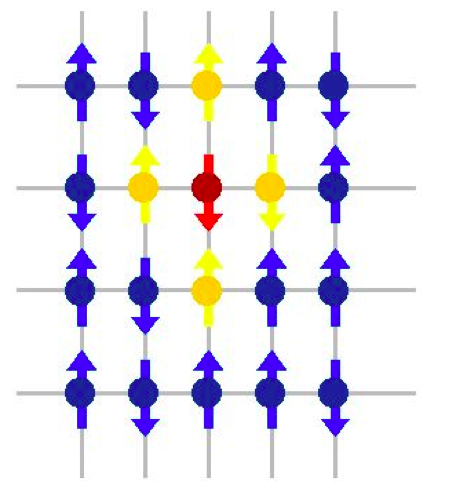
\includegraphics[height=150pt]{pics/ising2}
  \captionof{figure}{Graphical representation of the Ising model on a 2D square lattice.}
  \label{fig:ising}
\end{minipage}%
\hfill
\begin{minipage}{.48\textwidth}
  \centering
  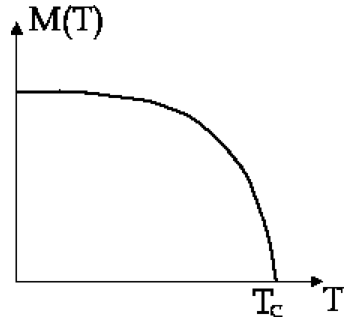
\includegraphics[height=150pt]{pics/spon_mag}
  \captionof{figure}{Spontaneous magnetization in the Ising model.}
  \label{fig:magnetization}
\end{minipage}
\end{minipage}
\vspace{0.1cm}



The simplest approach to the Ising model is imagining a squared lattice and assuming that every variable $\sigma_i \in \mkl{1,-1}$ on the lattice only affects the nearest neighbors (see Fig. \ref{fig:ising}). This restriction can be relaxed by letting the sites interact with the next nearest neighbors or even farther sites. If we think of the variables as spins, their interaction is given by the Hamiltonian 
\begin{equation}
\mathcal{H}\kl{X}=\underbrace{-J\sum_{i,j:\text{nn}}{\sigma_i\sigma_j}}_{A}\underbrace{-H\sum_{i=1}^N{\sigma_i}}_{B}.
\label{eq:hamiltonian}
\end{equation} where A is the interaction between all the nearest neighbors (nn), and B the interaction of each site with an external magnetic field $H$. Note that if two spins are parallel, then the energy is lowered ($-J$) and if they are anti-parallel the energy is increased ($+J$). 



The first term in Eq. \eqref{eq:hamiltonian} tries to create \emph{order} in the system (in the sense of the spins being aligned in the same direction) by reducing the energy when neighboring variables are in the same state. The second term tends to align the spins in the direction of the external field $H$. While the energy is lower in an ordered state, the heat tends to destroy the order by flipping single spins. Beyond a critical temperature $T_c$ (i.e., for  $T>T_c$), the system is dominated by randomness and there is no alignment of the spins anymore. This transition, like any other phase transition (e.g. sol-gel transition) between ordered and disordered states, can be characterized by an \emph{order parameter}. In the case of the Ising model, the order parameter is given by the spontaneous magnetization (see Fig. \ref{fig:magnetization}).


\subsubsection*{The order parameter in the Ising model}
The magnetization is defined as 
\begin{equation}
M\kl{T} =   \avkl{\frac{1}{N} \sum_{i=1}^N{\sigma_i} } ,
\end{equation} that is, the thermal average of the mean value of the spins. This alone would not be  a good measure since taking the thermal average of a quantity means taking the mean value over all the possible states. The problem with this procedure is that for any given state there will always exist an opposite state in which all the spins are flipped. In the average these two configurations cancel each other out. Thus, on average, every state will always cancel out with its opposite companion and the averaged magnetization will always be zero. A better quantity is the \emph{spontaneous magnetization}: 
\begin{equation}
M_\text{S}\kl{T} \equiv \lim_{\vec{H}\rightarrow 0}{  \avkl{\frac{1}{N} \sum_{i=1}^N{\sigma_i} }  }
\label{eq:spon_magn}
\end{equation}
Here the symmetry of the Ising model is broken by applying a small field $\vec{H}$ that aligns the spins in one direction. Now it will not be the same if the spins are up or down, and the thermal average of the spontaneous magnetization won't be zero anymore. Another way of breaking the symmetry would be fixing the boundaries of the lattice in a certain state. This is not practical if periodic boundaries are being used.

In the proximity of the critical temperature, the spontaneous magnetization decays like a power law: 
\begin{equation}
M_\text{S} \propto \kl{T-T_c}^\beta,
\label{eq:powerlaw_unfortunate}
\end{equation}
where $\beta$ is known analytically in 2D (1/8), and numerically in 3D ($\approx 0.326$) (See Fig. \ref{fig:magnetization}).

\subsubsection*{Response functions:}
Response functions are second derivatives of the free energy\footnote{The following established nomenclature is unfortunate: with $\beta$, the thermodynamical quantity $\frac{1}{k_BT}$ is meant, not the exponent presented in the power law \eqref{eq:powerlaw_unfortunate}. See classical statistical physics textbooks for more information.} $E_f = -\frac{1}{\beta} ln \kl{Z}$:

\begin{equation}
\chi\kl{T} \equiv \pder{M}{H}\bigg| _{T,H=0} \propto \abs{T-T_c}^{-\gamma}
\label{eq:susce}
\end{equation}
\begin{equation}
C_{\text{V}}\kl{T} \equiv \pder{E}{T}\bigg| _{H=0} \propto \abs{T-T_c}^{-\alpha}
\end{equation}
The divergence of these functions at the critical temperature can be used to determine the critical temperature itself. We will encounter these functions again later in the context of the $n^{th}$ \emph{order transition} (see Sec. \ref{subsec:first_order_trans}).


\subsubsection*{Fluctuation-dissipation theorem for the magnetic susceptibility:}
Taking equation \eqref{eq:spon_magn}, and plugging it into Eq. \eqref{eq:susce} yields
\begin{equation*}
\chi \kl{T}   =
 \left.\pder{\avkl{M\kl{T,H}}}{H} \right|_{H=0} =
  \pder{}{H} \left.\frac { \sum_X{\sum_{i=1}^N{\sigma_i \exp\ekl{H_0+\beta H \sum_{i=1}^N{\sigma_i}}}}}   {\underbrace   {\sum_X{ \exp\ekl{H_0+\beta H \sum_{i=1}^N{\sigma_i}}}}_{= Z_T\kl{H}}}\right|_{H=0}
\end{equation*}
with $\beta = \frac{1}{k_BT}$ and $H_0=\beta J \sum_{i,j:nn}{\sigma_i\sigma_j}$. Using the product rule yields:
  

\begin{align*}
\chi \kl{T}   &=  \left. \underbrace{\frac   {\beta \sum_X{\kl{\sum_{i=1}^N{\sigma_i} }}^2  \exp\ekl{H_0+\beta H \sum_{i=1}^N{\sigma_i}}  }     {Z_T\kl{H}} }  
-
 \underbrace{\frac   {\beta\kl{ \sum_X{\sum_{i=1}^N{\sigma_i} }  \exp\ekl{H_0+\beta H \sum_{i=1}^N{\sigma_i}} }^2 }    { \kl{Z_T\kl{H}}^2 }} \right| _{H=0}  \\
&=  \hspace{2.4cm} \beta  \avkl{M\kl{T}^2} \hspace{2.7cm} -\hspace{2.6cm}\beta\avkl{M\kl{T}}^2   
\end{align*}
\begin{equation}
\hspace{-7.5cm}=\beta\ekl{ \avkl{M\kl{T}^2}  -  \avkl{M\kl{T}}^2    }\ge 0 \hfill
\end{equation}

\vspace{0.2cm}
and analogously one can show that

\begin{equation}
C_\text{V}=\beta^2 \ekl{    \avkl{E\kl{T}^2}  -\avkl{E\kl{T}}^2  } 
\end{equation} 


You may have already noticed that these expressions are suspiciously similar to the classical definition of the variance. These two last formulae are both very important in Monte Carlo simulations, as we will learn further on.  See Fig. \ref{fig:susce}, \ref{fig:spec_heat}, and \ref{fig:corr_len}.
In the vicinity of $T_c$ (see Fig. \ref{fig:susce}), the magnetic susceptibility decays like a power law: 
\begin{equation*}
\chi \kl{T} \propto \abs{T-T_c}^{-\gamma}
\end{equation*}
with $\gamma$ =7/4 in 2D and $\approx 1.24$ ind 3D.  Near $T_c$ (see Fig. \ref{fig:spec_heat}), the specific heat can also be described by a power law:
\begin{equation*}
C_\nu \kl{T} \propto \abs{T-T_c}^{-\alpha}
\end{equation*}
where the decay is logarithmic in 2D ($\alpha$= 0) and numerically known in 3D ($\alpha$$\approx$ 0.11).

\vspace{0.1cm}


\begin{comment}
\begin{figure}
		\centering
        \begin{subfigure}[b]{0.45\textwidth}
                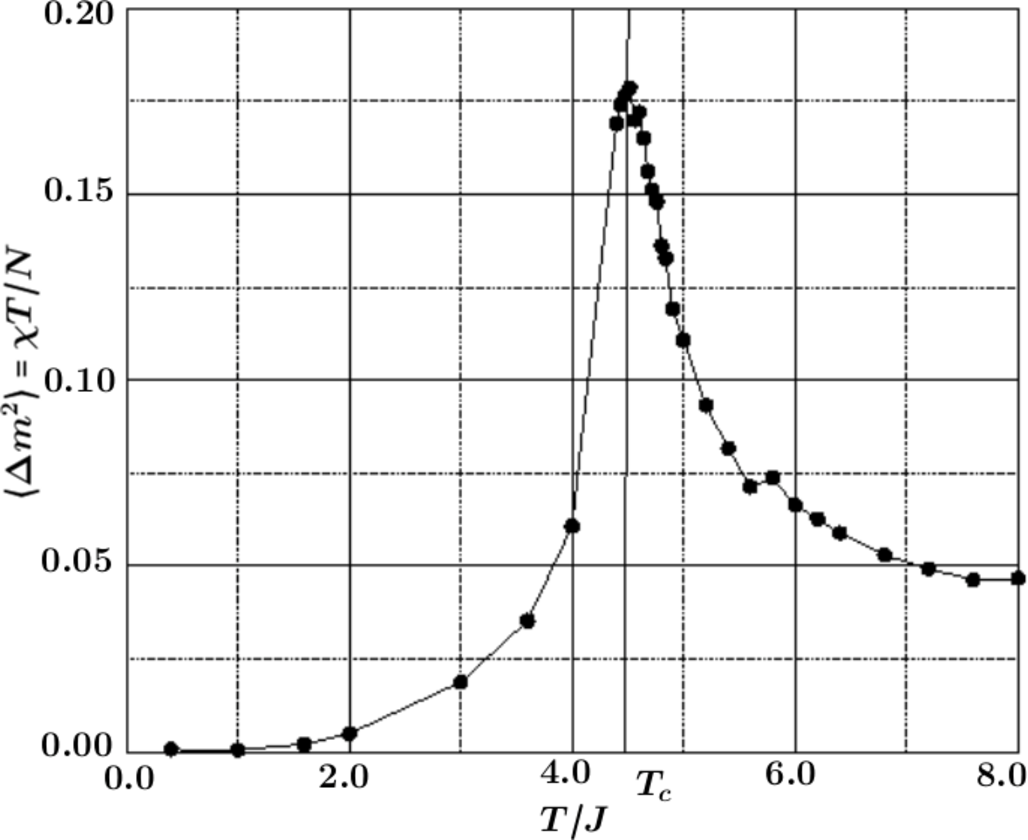
\includegraphics[width=\textwidth]{pics/susce_nottitle.pdf}
                \caption{Susceptibility in a finite system}
                \label{fig:susce}
        \end{subfigure}%
~
       \begin{subfigure}[b]{0.45\textwidth}
                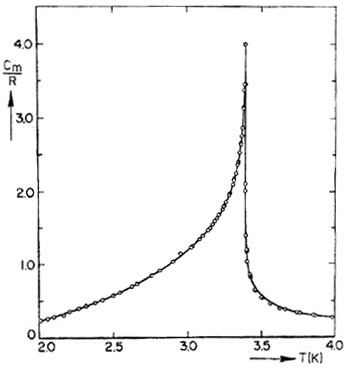
\includegraphics[width=\textwidth]{pics/heat_cap_MIT.jpg}
                \caption{Heat capacity of a binary mixture. Retr. Jan 2015 from web.mit.edu/8.334/www/grades/projects/}
                \label{fig:spec_heat}
        \end{subfigure}
        \caption{Pictures of animals}
	\label{fig:animals}
\end{figure}
\end{comment}



\begin{minipage}{\textwidth}
\begin{minipage}{.5\textwidth}
  \centering
  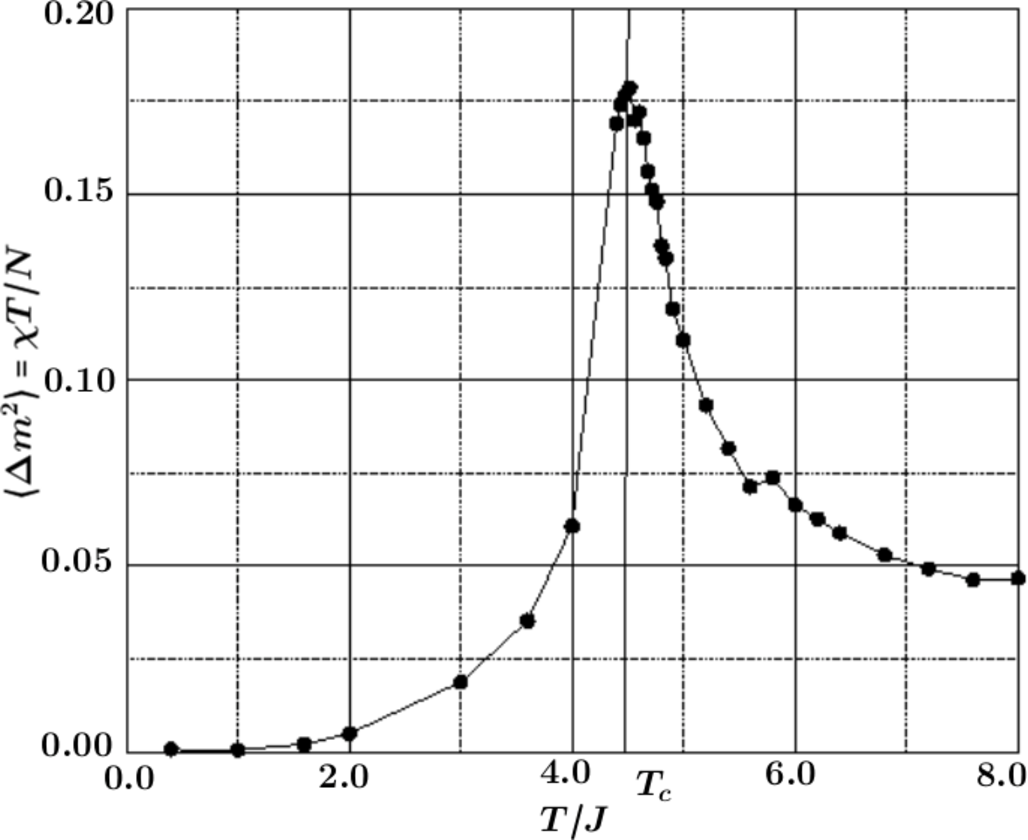
\includegraphics[width=0.95\textwidth]{pics/susce_nottitle.pdf}
  \captionof{figure}{Susceptibility in a finite system}
  \label{fig:susce}
\end{minipage}
\hfill
\begin{minipage}{.5\textwidth}
  \centering
  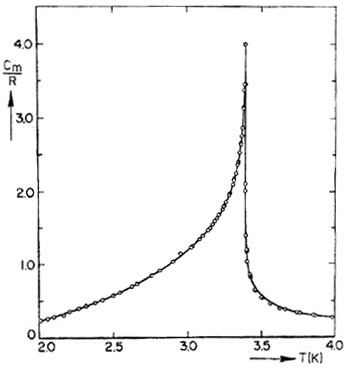
\includegraphics[width=0.95\textwidth]{pics/heat_cap_MIT.jpg}
  \captionof{figure}{Heat capacity of a binary mixture. Retr. Jan 2015 from web.mit.edu/8.334/www/grades/projects/}
  \label{fig:spec_heat}
\end{minipage}
\end{minipage}
\vspace{0.1cm}


\subsubsection*{Correlation length\footnote{See Fig. \ref{fig:corr_len} and the lecture notes \emph{Computational Physics} of the previous course.}}


\begin{wrapfigure}{r}{0.5\textwidth}
  	\begin{center}
    	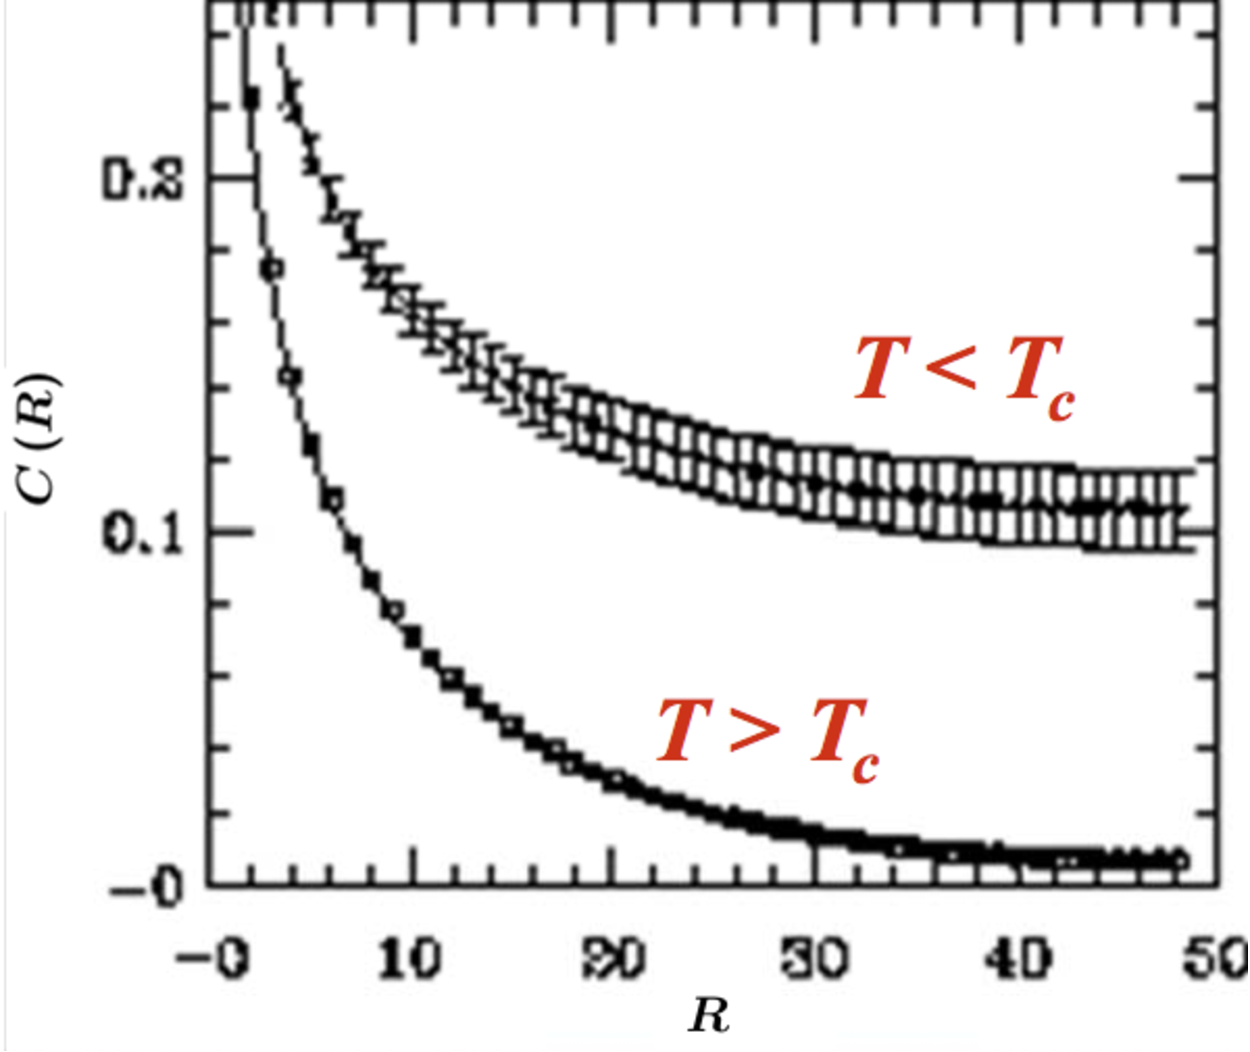
\includegraphics[width=0.4\textwidth]{pics/corr_len.pdf}
		\label{fig:corr_len}
  	\end{center}
  	\caption{Correlation in finite system}
\end{wrapfigure}


The correlation function describes to which extent two sites (or extended regions) are related. It is defined by the thermal average of the product of  the values of sites at different positions:
	\begin{equation}
C(R) \equiv \avkl{\sigma\kl{0}\sigma\kl{R}}.
		\label{eq:corr_len}
	\end{equation}
If two regions are exactly in the same physical state, the correlation function is maximized. This function decays exponentially for large $R$: 
	\begin{equation*}
C(R) \propto M^2 + a e^{-\frac{R}{\xi}}
	\end{equation*}
where $\xi$ is called the \emph{correlation length}.


\begin{comment}
\begin{minipage}{\textwidth}
	\begin{minipage}{.48\textwidth}
The correlation function describes to which extent two sites (or extended regions) are related. It is defined by the thermal average of the product of  the values of sites at different positions:
	\begin{equation}
C(R) \equiv \avkl{\sigma\kl{0}\sigma\kl{R}}.
		\label{eq:corr_len}
	\end{equation}
If two regions are exactly in the same physical state, the correlation function is maximized. This function decays exponentially for large $R$: 
	\begin{equation*}
C(R) \propto M^2 + a e^{-\frac{R}{\xi}}
	\end{equation*}
where $\xi$ is called the \emph{correlation length}.
	\end{minipage}%
	\hfill
	\begin{minipage}{.5\textwidth}
  		\centering
  		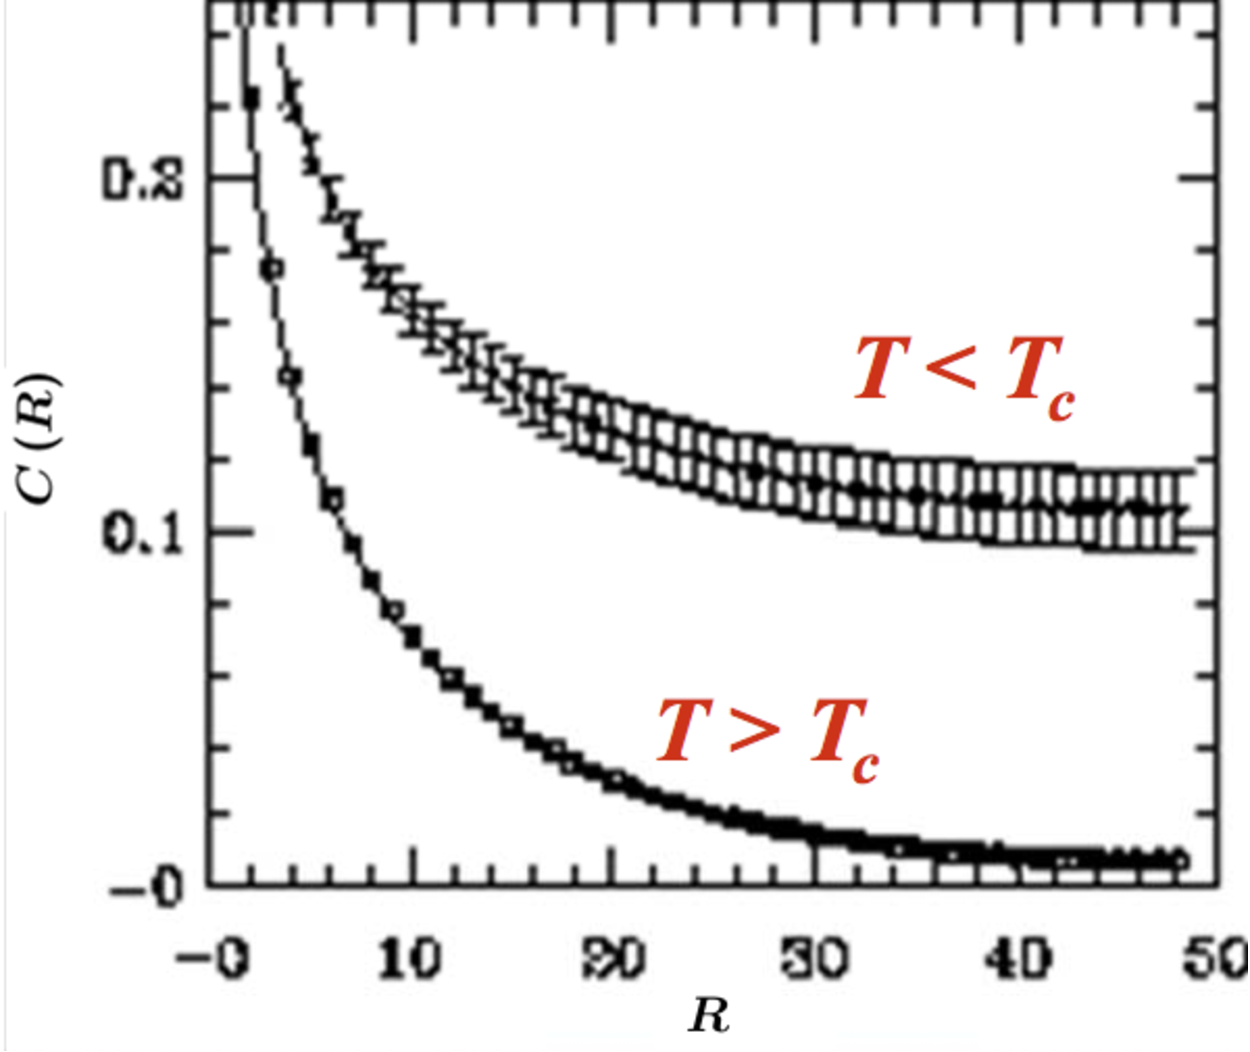
\includegraphics[width=0.95\textwidth]{pics/corr_len.pdf}
  		\captionof{figure}{Correlation in finite system}
  		\label{fig:corr_len}
	\end{minipage}
\end{minipage}
\end{comment}


\vspace{0.1cm}

\noindent
In the vicinity of $T_c$ the correlation length $\xi$ diverges as $$\xi \propto \abs{T-T_c}^{-\nu}$$ with $\nu = 1$ in 2D and $\nu\approx 0.63$ in 3D. At $T_c$ and for large R, we have that $$C(R) \propto R^{2-d-\eta},$$ where d is the dimensionality of the system and $\eta$ = 1/4 in 2D and $\eta\approx0.05$ in 3D.





\subsubsection*{Critical Exponents:}

All the quantities described in Figs. \ref{fig:susce}, \ref{fig:spec_heat} and \ref{fig:corr_len} are characterized by some exponents ($\alpha$, $\beta$, $\gamma$, $\eta$ and $\nu$). An interesting fact is that these exponents are not independent from each other. They are related by the \emph{scaling} and the \emph{hyperscaling} relations \footnote{For more information about these the exponents, see \citet{scaling_stanley} and \citet{stanley}}:

$$\alpha + 2\beta + \gamma =2$$
$$ 2-\alpha =d\nu$$
\begin{equation}(2-\eta)\nu=\gamma\end{equation}
Due to these relations, the number of independent exponents reduces to two.





